%%%% imav.tex
% This is the tex-file for the IMAV 2014 conference
% for questions / remarks / bugs regarding the files, please contact info@imavs.org
% You can use this style for your conference, as long as you refer to the IMAV 2014
% in a comment similar to this one.
% Of course, the IMAV 2014 is not liable for any aspects of its use.

\documentclass{article}
% The style file
\usepackage{imav}
% Use the postscript times font!
\usepackage{times}
\usepackage{graphicx}
\usepackage{algorithm}
\usepackage{algorithmic}
\usepackage{wasysym}
%\numberwithin{algorithm}{chapter}
%\usepackage{algorithmicx}
% the following package is optional:
%\usepackage{latexsym}

\title{Article Template for IMAV 2014}
\author{A. AuthorName1\thanks{Email address(es): contact\_author@mail.com}, S.B. AuthorName2, and C. AuthorName3 \\ University of A, Z road, Paysana}

\begin{document}

\maketitle

\begin{abstract}
This is the article template for the IMAV 2014 to be used with Latex. The abstract should contain a short description of the research. It can maximally be 300 words.
\end{abstract}

\section{Introduction} \label{section:introduction}
In Latex, you do not have to worry much about the style. It is best to use the `imav\_template.tex'-file as a template. Just remove our text and put your text in its place. Copy the code for figures and tables, and put your data in them. Most comments in this document are best understood by looking at the latex source file. We include a `build.bat' file that transforms the tex-file into a pdf. 

\section{Figures and Tables}
\subsection{Figures}
To insert images in Latex, use the template below. The figure caption should be below the figure. Images can be included in colour, since the proceedings will only be released in digital form. 

\begin{figure}[hbt]
\centering
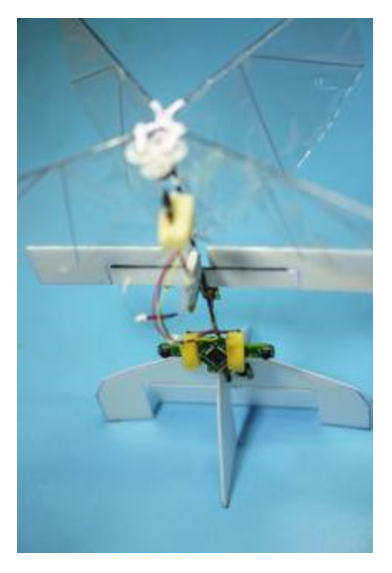
\includegraphics[width=4cm]{DelFlyExplorer.eps}
\caption{Be sure to select the figure caption style.}
\label{figure:DelFly_Explorer}
\end{figure}

\subsection{Tables}
When inserting a table, you can choose the appropriate style - below is an example. Put the caption under the table.

\begin{table}[hbt]
\begin{center}
\begin{tabular}{|l|c|c|c|}
\hline
& A & B& C\\
\hline
X & 1 & 2 & 3\\
Y & 1 & 2 & 3\\
\hline
\end{tabular}
\caption{Results of the experiment.}
\label{table:results}
\end{center}
\end{table}

\section{Math and Units}

\subsection{Math}
Include equations in Latex with the equation environment:

\begin{equation} \label{equation:n}
n = \sqrt{\frac{a}{b}}
\end{equation}

If used inside the text, use the \$-sign: $a =  b-c$. Only do this for short formulas.

\subsection{Units}
Always use SI units first, possibly adding other units in parentheses.

\section{Referencing}

\subsection{In-document referencing}
Always introduce a figure as 'Figure X', as in "Figure \ref{figure:DelFly_Explorer} shows the DelFly Explorer.", or "The DelFly Explorer is shown in Figure \ref{figure:DelFly_Explorer}." Subsequently, the word 'figure' can be used. The same goes for tables ('Table \ref{table:results}'). Equations do not have to be introduced this way. If they are referenced to, 'Equation \ref{equation:n}' should be used. Sections are referred to as 'Section \ref{section:introduction}'\footnote{Footnotes are placed like this.}

\subsection{Referencing to literature}
 Citations are numbered consecutively with square brackets \cite{DEWAGTER2014} - this is determined by the bibliography style `unsrt'. The references can be described in bibtex format in a separate bib-file (see the bibliography statement close to the end of the tex-file).  The sentence punctuation follows the brackets \cite{NOLFIPOWLIM}. Multiple references \cite{DEWAGTER2014,NOLFIPOWLIM} are each numbered with separate brackets or in sequence as \cite{DEWAGTER2014,NOLFIPOWLIM,BISHOP2006}.
Follow the reference style at the end of this document. Papers that have not been published should be cited as "unpublished". Papers that have been submitted for publication should be cited as "submitted for publication". Papers that have been accepted for publication, but not yet specified for an issue should be cited as "to appear". Capitalize only the first word in a paper title, except for proper nouns and element symbols.
Below, \cite{DEWAGTER2014} is a reference to a conference paper, \cite{NOLFIPOWLIM} to a journal paper, and \cite{BISHOP2006} to a book.

\section{Publishing Policy}
The IMAV proceedings will only be distributed in digital form. The submitting author is responsible for obtaining agreement of all his / her coauthors and any consent required from sponsors before submitting a paper. The authors are obliged to cite relevant prior work.

\section{Conclusion}
Conclusion of the paper.

\section*{Acknowledgements}
Here you can place your acknowledgment.

% BIBLIOGRAPHY:
% use {unsrt}:
\bibliographystyle{unsrt}
\bibliography{imav_bibliography}

% The following lines are necessary for showing the appendices correctly, do not change!
\appendix
\newcommand{\appsection}[1]{\let\oldthesection\thesection
  \renewcommand{\thesection}{Appendix \oldthesection:}
  \section{#1}\let\thesection\oldthesection}
% appendices are now indicated by appsection:

\appsection{Data}
If appendices are necessary, they appear at the end of the document. Use `appsection' instead of `section'.
\appsection{More data}
Even more data.
\end{document}

